\documentclass[10pt,a4paper]{article}
\usepackage[utf8]{inputenc}
\usepackage[german]{babel}
\usepackage{amsmath}
\usepackage{amsfonts}
\usepackage{amssymb}
\usepackage{siunitx}
\usepackage{multirow}
\usepackage[left=2cm,right=2cm,top=2cm,bottom=2cm]{geometry}
\usepackage{wrapfig}
\usepackage{graphicx}
\usepackage[outdir=./]{epstopdf}
\usepackage{caption}
\usepackage[colorlinks]{hyperref}


\author{Christian Bespin \and Christopher Deutsch}
\title{Übungsblatt 3: Numerische Methoden der Physik}
\begin{document}
\maketitle

\setcounter{section}{1}

\section{Treibhauseffekt}

\subsection{Physikalischer Hintergrund}

Wir verwenden zur Erklärung des Treibhauseffektes ein einfaches Modell grauer und schwarzer Körper. Die Erde entspricht dabei einem schwarzen Körper, das heißt Emissionsgrad ist gleich $1$, mit der Temperatur $T_E$. Die Sonne wird als grauer Körper mit konstanter Emissivität $\epsilon_S$ und ebenfalls konstanter Temperatur $T_S$. Im Gegensatz zum schwarzen Körper, absorbiert der graue Körper nicht die gesamte auf ihn treffende Strahlung und emittiert entsprechend auch nicht die maximal mögliche Schwarzkörperstrahlung. Es gilt daher, dass $\epsilon_{S}<1$. Im verwendeten Modell hat die Atmosphäre die Emissivität $\epsilon$ und die Temperatur $\tau$. Die Atmosphäre absorbiert den Anteil $\epsilon(T_S)$ der von der Sonne emittierte Srahlung, lässt entsprechend den Anteil $1-\epsilon(T_S)$ dieser Strahlung zur Erde durch und emittiert selber eine Strahlung mit Anteil $\epsilon(\tau)$. Letzteres, sowie die zur Berechnung benötigten Formeln sind unter $(1)$-$(3)$ auf dem Aufgabenzettel zu finden.
\begin{wrapfigure}{L}[1pt]{0.47\textwidth}
\centering
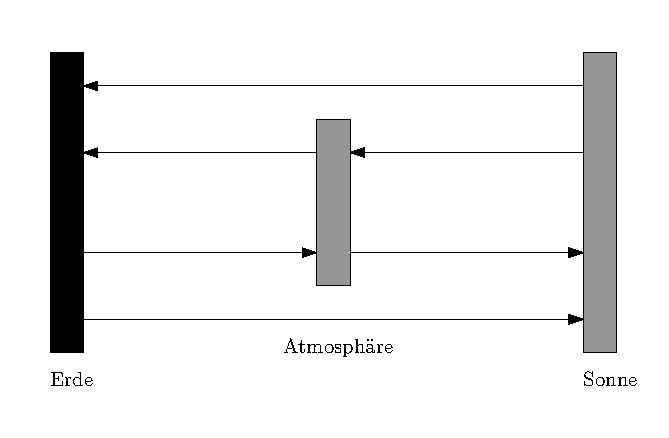
\includegraphics[width=0.45\textwidth]{./figures/strahlungsgleichgewicht.eps}
\caption{Strahlungsgleichgewicht}
\label{fig:strahlungsgleichgewicht}
\end{wrapfigure}
\\
Die Temperaturen der Körper ändern sich je nach abgestrahlter und emittierter Strahlung, bis sich irgendwann ein Strahlungsgleichgewicht einstellt. In diesem strahlen alle Körper genau so viel ab, wie sie absorbieren. Man kann für alle drei Elemente im Modell eine Formel aufstellen, die das Strahlungsgleichgewicht beschreibt. Dazu settz man an, dass die abgestrahlte Leistung $P$ proportional zu $\epsilon T^4$ ist (Stefan-Boltzmann-Gesetz). Weiterhin gilt nach Kirchhoff, dass die Absorptions- und Emissionskoeffizient eines Körpers gleich groß sind; es wird immer so viel Leistung emittiert, wie absorbiert. Damit erhält man für das Gleichgewicht der Atmosphäre (die Proportionalitätsfaktoren von $P$ werden vernachlässigt, sie kürzen sich beim Lösen heraus):
\begin{align}
2\epsilon(\tau)\tau^4=\epsilon(T_S)\epsilon_s T_S^4+\epsilon(T_E)T_E^4
\end{align}
Der Term auf der linken Seite beschreibt die von der Atmosphäre abgestrahlte Leistung. Der Faktor $2$ berücksichtigt die Abstrahlung sowohl zur Erde als auch zur Sonne. Die absorbierte Strahlung auf der rechten Seite setzt sich zusammen aus der von der Sonne und der Erde emittierten Strahlung ($\epsilon_S T_s^4$ bzw. $T_E^4$, da $\epsilon_{\mathrm{Erde}}=1$). Die Faktoren $\epsilon(T)$ beschreiben nach Kirchhoff nicht nur die Emissivität, sondern auch den Absorptionskoeffizienten der Atmosphäre. Sie ist in diesem Modell ein grauer Körper und absorbiert nur einen Teil, der auf sie treffenden Strahlung. Die Gleichungen für Sonne und Erde lassen sich analog aufstellen mit den gegebenen Informationen.
Aus den Gleichungen lässt sich $\tau$ eliminieren und man erhält $(4)$ vom Aufgabenblatt:
\begin{align}
\left[2-\epsilon(T_E)\right]T_E^4=\epsilon_S\left[2-\epsilon(T_S)\right]T_S^4
\label{eqn:gleichgewicht}
\end{align}
Um $T_E$ zu bestimmen, muss man \ref{eqn:gleichgewicht} umstellen, so dass sich ein Nullstellenproblem ergibt:
\begin{align}
\left[2-\epsilon(T_E)\right]T_E^4-\epsilon_S\left[2-\epsilon(T_S)\right]T_S^4=0
\label{eqn:nullstellenform}
\end{align}


$\nu_{max}=T\cdot 5,8789254\num{1E10}\si{\per\second}\si{\per\kelvin}$ \footnote{http://physics.nist.gov/constants, Wien frequency displacement law constant}
$Z=\frac{8}{15}\frac{\pi^5 \mathrm{kT}}{\mathrm{c}^3}$

\subsection{Mathematischer Hintergrund}

\subsection{Implementierung}

Das Programm besteht aus zwei Teilen: der numerischen Integration, bei der $epsilon(T)$ bestimmt wird und der numerischen Auswertung, um $T_E$ zu bestimmen, bei der \ref{eqn:nullstellenform} gilt.

Z wurde analytisch berechnet: 

\subsubsection{Nullstellenberechnung mit Bisektion}

Ein Verfahren, um numerisch Nullstellen zu bestimmen, ist das 1-Punkt-Iterationsverfahren Bisektion. Wir verwenden dieses hier, da es im Gegensatz zum Newtonverfahren keine Ableitungen der Funktion berechnen und auswerten muss. Dabei wird vorausgesetzt, dass die Funktion auf dem relevanten Intervall $[a,b]$ nur eine Nullstelle hat. Die Bisektion halbiert das zu betrachtende Intervall immer so, dass der Vorzeichenwechsel des Funktionswerts im betrachteten Intervall bleibt. Der Fehler halbiert sich mit jedem Iterationsschritt, was nicht so schnell wie das Newtonverfahren ist, die Laufzeit des Programms aber dennoch in einem akzeptablen Rahmen hält.
\begin{figure}[htbp]
\centering
\includegraphics[width=0.6\textwidth]{./figures/bisektion.eps}
\caption{Bisektions-Verfahren}
\label{fig:bisektion}
\end{figure}

\subsubsection{Numerische Integration mit rekursivem Simpson-Verfahren}

Wir verwenden zur numerischen Integration eine rekursive Variante des Simpson-Verfahrens, bei der das Intervall, über dem integriert wird, mit jedem Rekursionsschritt in zwei Hälften zerlegt wird, auf die die normale Simpson-Methode angewendet wird. Ist die Differenz zwischen dem mit Simpson über dem ganzen Intervall berechneten Integralwert und der Summe der zwei Teilintervalle größer als eine vorgegebene Genauigkeit, wird die Funktion rekursiv aufgerufen, wodurch jedes der Teilintervalle erneut halbiert wird. Durch dieses Vorgehen fallen im Gegensatz zum gewöhnlichen Simpsonverfahren einige laufzeitbeeinträchtigende Funktionsaufrufe weg.

\subsubsection{Abbruchbedingungen}

\subsubsection{Genaugkeit}

\subsection{Physikalische Ergebnisse}
\label{ssec:physikalischeergebnisse}

\begin{thebibliography}{9}

\bibitem{abramowitzstegun}
Abramowitz, M. \& Stegun, I. A.
\emph{Handbook of Mathematical Functions},
Dover Books (1965)

\bibitem{healdmarion}
Heald, M. \& Marion, J.
\emph{Classical Electromagnetic Radiation},
Brooks Cole (1994)

\bibitem{kazimierczuk}
Kazimierczuk, M.
\emph{High-Frequency Magnetic Components},
Wiley (2009)

\bibitem{crchandbook}
David R. Lide (ed),
\emph{CRC Handbook of Chemistry and Physics},
84th Edition. CRC Press. Boca Raton, Florida, 2003;
Section 12, Properties of Solids; Electrical Resistivity of Pure Metals;
Section 4, The Elements: Magnetic Susceptibility

\end{thebibliography}

\end{document}
